\chapter{Mengenal Kecerdasan Buatan dan Scikit-Learn}

\section{Teori}
Praktek teori penunjang yang dikerjakan :
\begin{enumerate}
	\item Sejarah Perkembangan dan penjelasan Definisi \textit{Artifical Intelligence}. \textit{Artifical Intelligence} merupakan suatu ilmu pada bidang komputer yang memiliki 
	kemampuan untuk meniru, melakukan sesuatu sama seperti yang dilakukan oleh manusia.\\
	Pada akhir tahun 1955 program \textit{Artifical Intelligence} pertama kali muncul berkat adanya perkembangan \textit{The Logic Theorist} oleh Newell dan Simon. 
	Program tersebut menunjukan masalah dengan menggunakan model pohon, dimana untuk menyelesaikannya hanya perlu memilih sebuah cabang yang akan menghasilkan sebuah kesimpulan yang paling
	benar. Dengan adanya program tersebut pengembangan dibidang  \textit{Artifical Intelligence} mengalami peningkatan yang besar. Di tahun 1956, seseorang bernama John McCarthy dari 
	Massacuhetts Institute of Technology yang juga dikenal sebagai Bapak AI, menyelenggarakan sebuah konferensi dengan nama \textit{The Dartmouth summer research project on artificial intelligence},
	konferensi itu diselenggarakan untuk menarik minat para ahli komputer untuk berkumpul dan bertemu. Konferensi tersebut mempertemukan para pendiri dibidang AI dan bertugas untuk meletakan
	dasar untuk penelitian dan pengembangan \textit{Artifical Intelligence} dimasa depan.
	
	\item Definisi supervised learning, klasifikasi, regresi dan unsupervised learning. Data set, training set dan testing set
	\begin{itemize}
		\item Supervised Learning
		\par
		\textit{Supervised learning}
		adalah suatu pendekatan machine learning yang ditentukan berdasarkan penggunaan dataset, supervised learning menggunakan dataset berlabel atau labeled dataset. Supervised Learning digunakan untuk melakukan klasifikasi data atau memprediksi hasil secara akurat sesuai dengan output berdasarkan pola yang ada didalam data training dan berupa data yang memiliki label yang sudah ditentukan terlebih dahulu
		\item Unsupervised Learning
		\par
		\textit{Unsupervised Learning} adalah pendekatan machine learning yang digunakan untuk menganalisa dan juga mengelompokan kumpulan - kumpulan data yang tidak berlabel.
		\item Klasifikasi
		\par
		\textit{Klasifikasi} adalah sebuah proses menggunakan algoritma untuk secara akurat memasukan data kedalam kategori yang spesifik.
		\item Regresi
		\par
		\textit{Regresi} adalah sebuah proses menggunakan algoritma untuk memahami hubungan antara 2 variabel, yaitu variabel dependen dan variabel independen, Regresi dapat memprediksi nilai numerik variabel dependen berdasarkan variabel independen.
		\item Dataset
		\par
		\textit{Dataset} adalah suatu kumpulan data yang berisi informasi-informasi lama, dan dapat dikelola sehingga menjadi sebuah informasi baru.
		\item Training set
		\par
		\textit{Training set} adalah bagian dari dataset yang dilatih untuk kemudian digunakan untuk memprediksi sesuatu atau menjalankan fungsi dari algoritma.
		\item Testing set
		\par
		\textit{Testing set} adalah bagian dari dataset yang digunakan untuk melihat tingkat keakuratan dan performa dari algoritma.
	\end{itemize}

\end{enumerate}


\section{Instalasi}

\begin{enumerate}
\item Melakukan installasi pada anaconda promt dengan perintah " pip install -U scikit-learn".
\begin{figure}[!htbp]
	\centering
	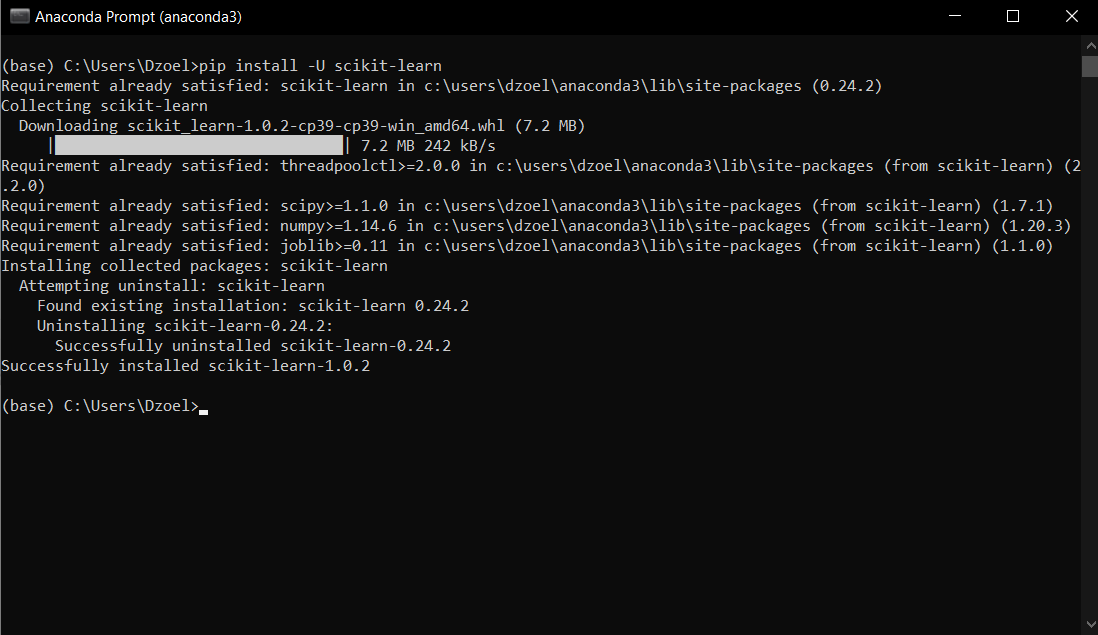
\includegraphics[scale=0.4]{figures/pipinstall.PNG}
\end{figure}
\newpage
\item Kemudian klik link berikut ini untuk melakukan basic tutorial \textit{scikit-learn} "https://scikit-learn.org/stable/tutorial/basic/tutorial.html".
\item
Mencoba Loading an example dataset
\begin{figure}[!htbp]
	\centering
	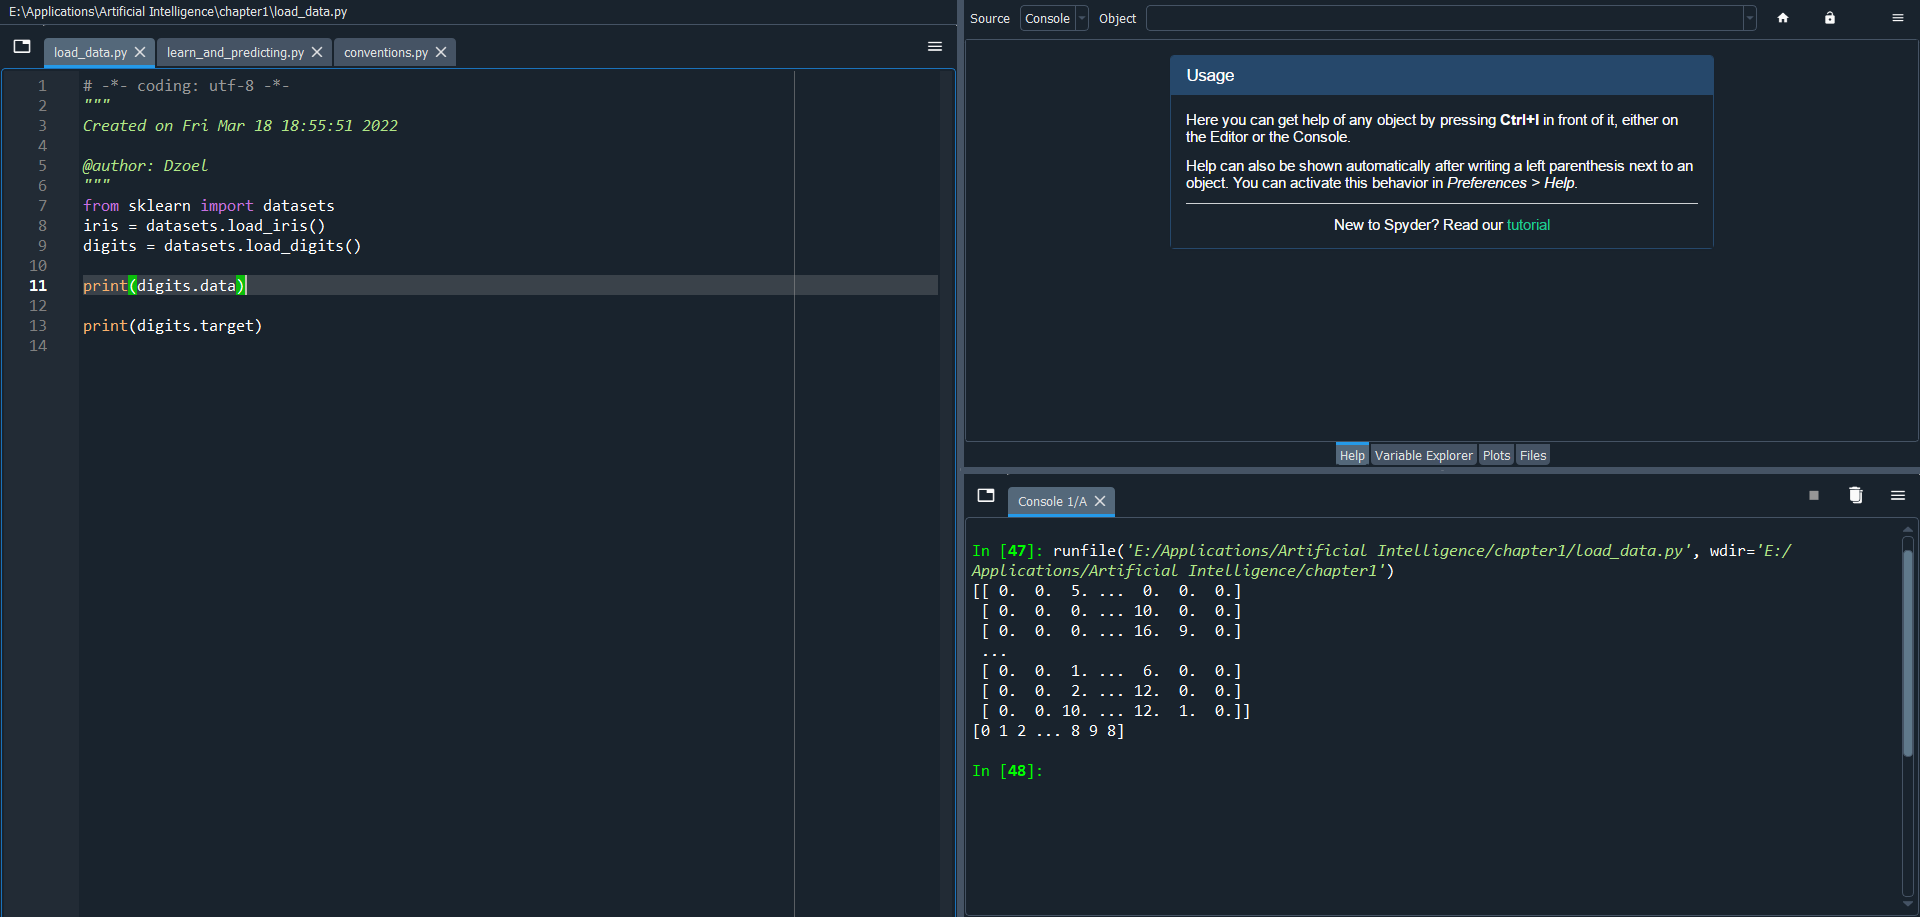
\includegraphics[scale=0.4]{figures/loaddataset.PNG}
\end{figure}
\item
Mencoba Learning and predicting
\begin{figure}[!htbp]
	\centering
	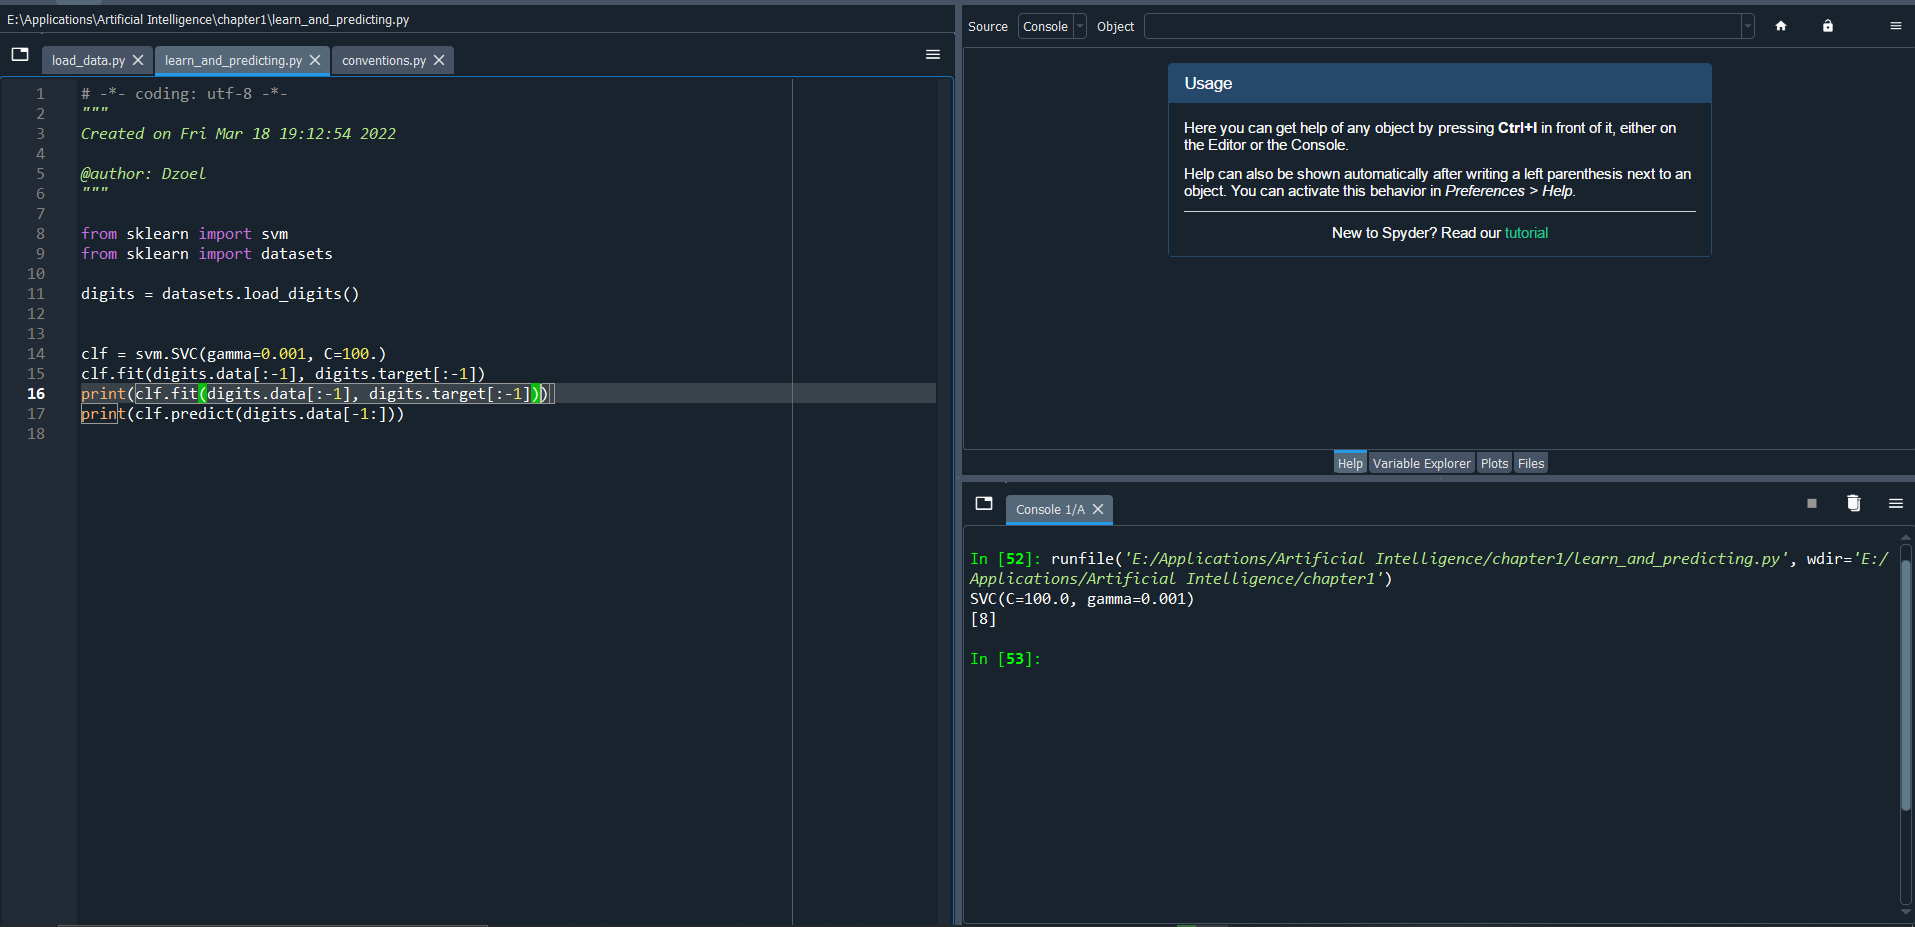
\includegraphics[scale=0.4]{figures/learnpredict.PNG}
\end{figure}
\newpage
\item 
Mencoba Conventions
\begin{figure}[!htbp]
	\centering
	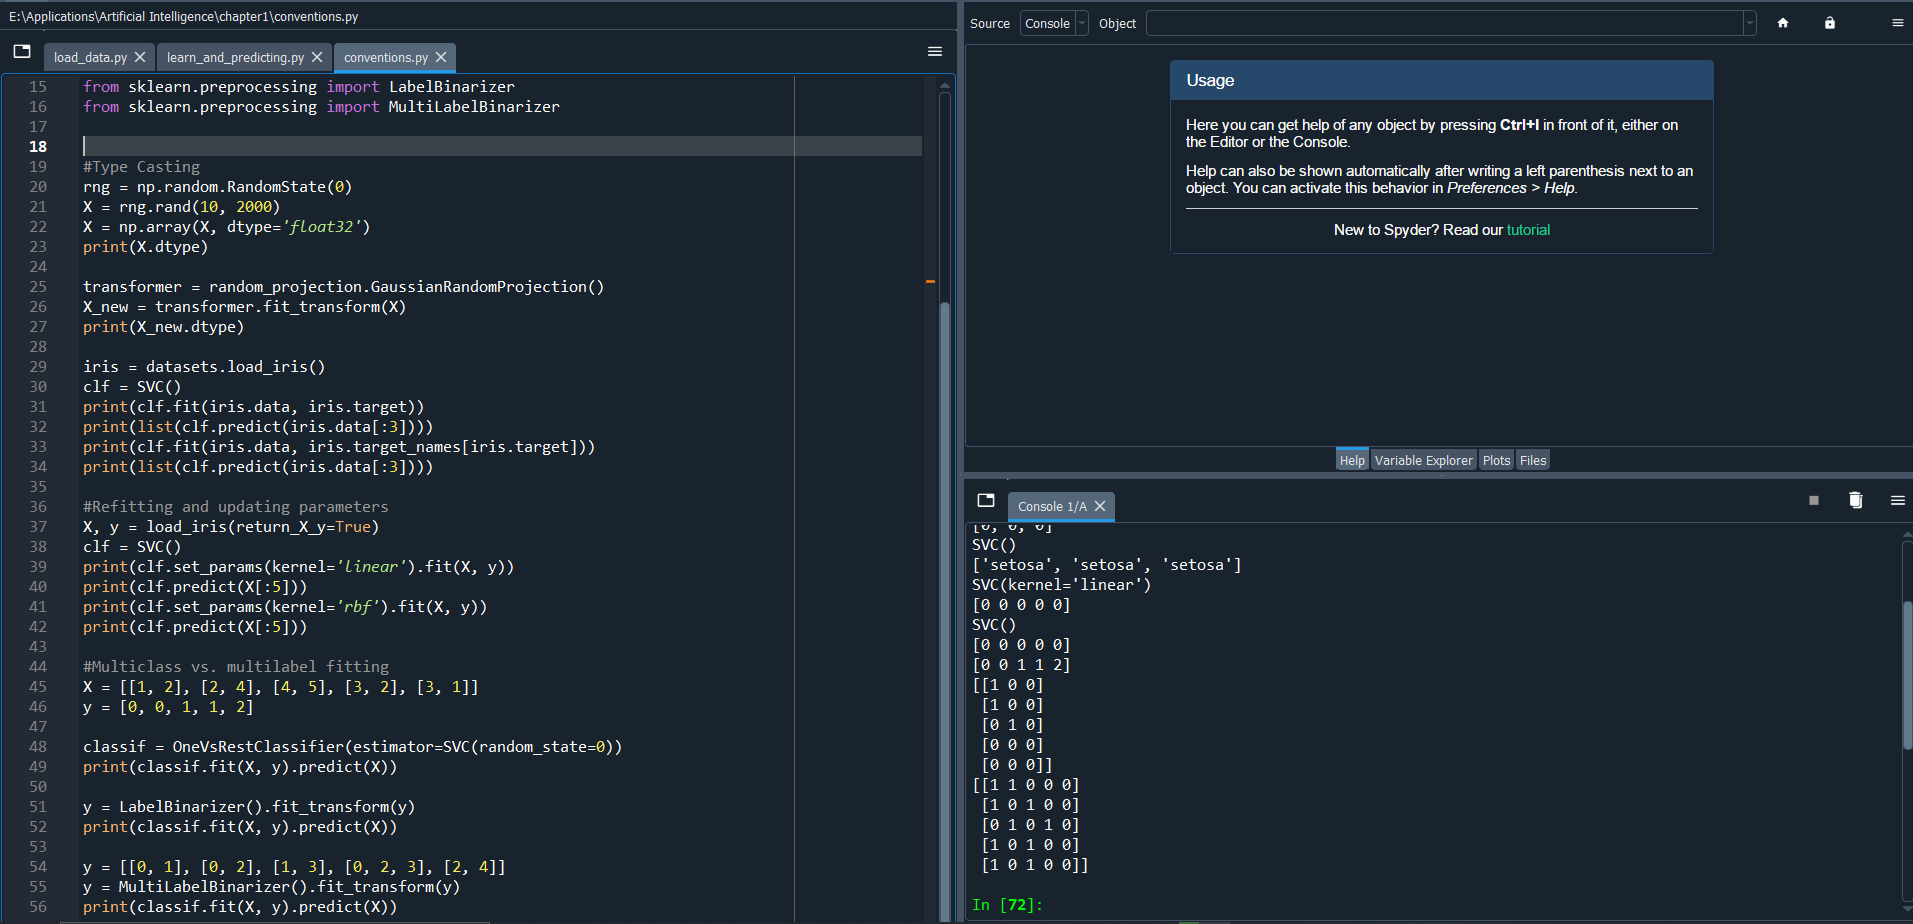
\includegraphics[scale=0.4]{figures/convention.PNG}
\end{figure}
\newpage
\item Link Youtube praktikum : https://www.youtube.com/watch?v=tFsRdpQ-VUg
\end{enumerate}


\section{Penanganan Error}
Dari percobaan yang dilakukan di atas, apabila mendapatkan error maka:

\begin{enumerate}
\item Screenshoot Error
\begin{figure}[!htbp]
	\centering
	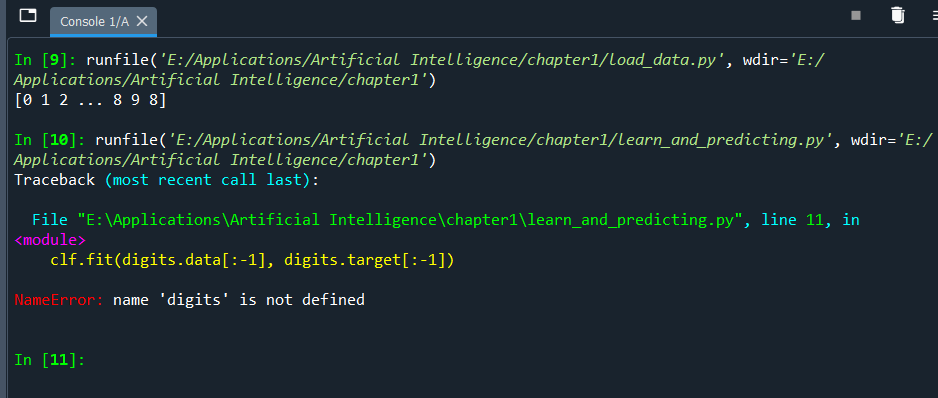
\includegraphics[scale=0.6]{figures/nameError.PNG}
\end{figure}
\begin{figure}[!htbp]
	\centering
	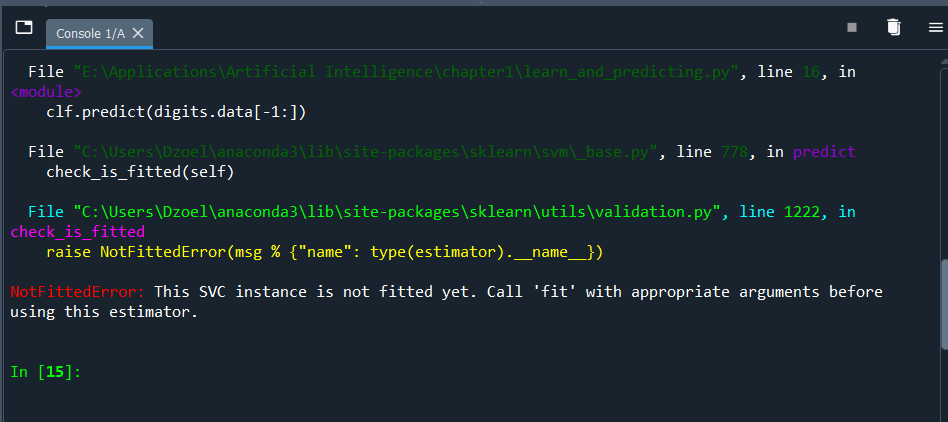
\includegraphics[scale=0.6]{figures/notfittederror.PNG}
\end{figure}

\newpage    
\item Tuliskan kode error dan jenis error
\par 
NameError = name 'digits' is not defined
\par
NotFittedError = This SVC instance is not fitted yet. Call 'fit' with appropriate arguments before using this estimator.

	\item
Solusi pemecahan masalah error tersebut
\par
NameError = solusinya adalah membuat variabel dengan nama digits
\par
NotFittedError = solusinya adalah memanggil parameter dengan method fit, sebelum menggunakan method predict.

\end{enumerate}

